\epigraph{Many C programmers believe that ``strong typing''
          just means pounding extra hard on the keyboard.
}
{--- \textup{Peter van den Linden}}

Dans ce chapitre, nous enrichissons le langage défini dans le
chapitre~\ref{cha:lang} d'un système de types. Celui-ci permet de séparer les
programmes bien formés, comme celui de la figure~\ref{fig:progwf:good} des
programmes mal formés comme celui de la figure~\ref{fig:progwf:bad}.

\begin{SaveVerbatim}[]{VerbProgGood}
f()
(x=0)
{
  x = 1
  return x
}
\end{SaveVerbatim}

\begin{SaveVerbatim}[]{VerbProgBad}
f()
(x=0)
{
  x = 1
  return (*x)
}
\end{SaveVerbatim}

\begin{figure}

  \centering

  \subbottom[Programme bien formé]{
\label{fig:progwf:good}
    \BUseVerbatim{VerbProgGood}
  }
  \hspace{2cm}
  \subbottom[Programme mal formé]{
\label{fig:progwf:bad}
    \BUseVerbatim{VerbProgBad}
  }

  \caption{Programmes bien et mal formés}
\label{fig:progwf}

\end{figure}

Le but d'un tel système de types est de rejeter les programmes qui sont
``évidemment faux'', c'est-à-dire dont on peut prouver qu'il provoqueraient des
erreurs à l'exécution dues à une incompatibilité entre valeurs. En ajoutant
cette étape, on restreint la classe d'erreurs qui pourraient bloquer la
sémantique.

\section{Principe}

Le principe est d'associer à chaque construction syntaxique une étiquette
représentant le genre de valeurs qu'elle produira. Dans le programme de la
figure~\ref{fig:progwf:good}, la variable $x$ est initialisée avec la valeur
$0$, c'est donc un entier. Cela signifie que dans tout le programme, toutes les
instances de cette variable
\footnote{Deux variables peuvent avoir le même nom dans deux fonctions
  différentes, par exemple. Dans ce cas il n'y a aucune contrainte particulière
  entre ces deux variables. L'analyse de typage se fait toujours dans un
  contexte précis.
}
porteront ce type. La première instruction est l'affectation de la constante $1$
(entière) à $x$ dont on sait qu'elle porte des valeurs entières, ce qui est donc
correct. Le fait de rencontrer $\iReturn{x}$ permet de conclure que le type de
la fonction est $() → \tInt$.

Dans la seconde fonction, au contraire, l'opérateur $*$ est appliqué à $x$ (le
début de l'analyse est identique et permet de conclure que $x$ porte des valeurs
entières). Or cet opérateur prend un argument d'un type pointeur de la forme
$t*$ et renvoie alors une valeur de type $t$. Ceci est valable pour tout $t$
($\tInt$, $\tFloat$ ou même $t'*$: le déréférencement d'un pointeur sur pointeur
donne un pointeur), mais le type de $x$, $\tInt$, n'est pas de cette forme. Ce
programme est donc mal typé.

\section{Environnements et notations}

\begin{figure}

  \begin{align*}
  \gramdef{Type}{t}
      { \tInt                       }{Entier}
      { \tFloat                     }{Flottant}
      { \tUnit                      }{Unité}
      { t*                          }{Pointeur}
      { t[]                         }{Tableau}
      { S                           }{Structure}
      { (t_1, …, t_n) \rightarrow t }{Fonction}
      {END} \\
  \\
  \gramdef{Structure}{S}
      { \eStruct{ l_1 : t_1; … ; l_n : t_n } }{Structure simple}
      {END} \\
  \\
  \gramdef{Environnement de typage}{Γ}
      { []         }{Environnement vide}
      { (a, t)::Γ' }{Extension}
      {END}
  \end{align*}

  \caption{Types et environnements de typage}

\label{fig:les-types}

\end{figure}

Les types associés aux expressions sont décrits dans la
figure~\ref{fig:les-types}. Tous sont des types concrets: il n'y a pas de
polymorphisme.

Pour maintenir les contextes de typage, un environnement $Γ$ associe un type à
un ensemble de variables.

Plus précisément, un environnement $Γ$ est une liste de couples (variable,
type), c'est à dire une suite finie ${(γ_i)}_{i∈[1;n]}$ avec $γ_i = (x_i, t_i)$.
On utilise les notations suivantes:

\begin{align*}
  x:t ∈ Γ &\eqdef ∃i ∈ [1;n], γ_i = (x, t) \\
  \cDom{Γ} &\eqdef \{ x_i / i ∈ [1;n] \} \\
  Γ, x:t  &\eqdef {(γ'_i)}_{i∈[1;n+1]}~\textrm{tel que}
                        \begin{cases}
                          ∀ i ∈ [1;n], γ'_i    = γ_i \\
                                       γ_{n+1} = (x,t) \\
                        \end{cases} \\
  Γ - x   &\eqdef {(γ'_i)}_{i∈[1;n-1]}~\textrm{tel que}
                        \begin{cases}
                          ∀ i ∈ [1;p-1], γ'_i = γ_i \\
                          ∀ i ∈ [p;n-1], γ'_i = γ_{i+1} \\
                        \end{cases}
                        \mbox{ où } γ_p = (x, t_p)
\end{align*}

Par exemple, $(p, \tInt*) ∈ Γ$ permet de typer (sous $Γ$) l'expression $p$ en
$\tInt*$, $*p$ en $\tInt$ et $p +_p 4$ en $\tInt*$.

Le type des fonctions semble faire apparaître un n-uplet $(t_1, …, t_n)$ mais ce
n'est qu'une notation: il n'y a pas de n-uplets de première classe, ils sont
toujours présents dans un type fonctionnel.

\paragraph{Typage d'une expression:} on note de la manière suivante le fait
qu'une expression $e$ (telle que définie dans la figure~\ref{fig:stx-data}) ait
pour type $t$ dans le contexte $Γ$.

  \[
    \ty{Γ}{e}{t}
  \]

\paragraph{Typage d'une instruction:} les instructions n'ont en revanche pas de
type. Mais il est tout de même nécessaire de vérifier que troutes les
sous-expressions apparaissant dans une instruction sont cohérentes ensemble.

On note de la manière suivante le fait que sous l'environnement $Γ$
l'instruction $i$ est bien typée:

  \[
    \tyi{Γ}{i}
  \]

\paragraph{Typage d'une phrase:} De par leur nature séquentielle, les phrases
qui composent un programme altèrent l'environnement de typage. Par exemple, la
déclaration d'une variable globale ajoute une valeur dans l'environnement.

On note

  \[
    \typh{Γ}{p}{Γ'}
  \]

si le typage de la phrase $p$ transforme l'environnement $Γ$ en $Γ'$.

On étend cette notation aux suites de phrases, ce qui définit le typage d'un
programme, ce que l'on note $⊢ P$ (figure~\ref{fig:typ-suite-phrases}).

\begin{figure}
  \ruleheader{$\typhstar{Γ}{ps}{Γ'}$}

  \begin{mathpar}
    \irule{T*-Nil}
      { }
      { \typhstar{Γ}{[~]}{Γ} }

    \irule{T*-Cons}
      { \typh{Γ_1}{p}{Γ_2}
     \\ \typhstar{Γ_2}{ps}{Γ_3}
      }
      { \typhstar{Γ_1}{p::ps}{Γ_3} }
  \end{mathpar}

  \ruleheader{$Γ ⊢ P$}

  \begin{mathpar}
    \irule{Prog}
      { \typhstar{[~]}{P}{Γ} }
      { ⊢ P }
  \end{mathpar}

  \caption{Typage d'une suite de phrases et d'un programme}
\label{fig:typ-suite-phrases}
\end{figure}

\section{Expressions}

\subsection*{Littéraux}

Le typage des littéraux numériques ne dépend pas de l'environnement de typage:
ce sont toujours des entiers ou des flottants.

\begin{mathpar}

  \disprule{Cst-Int}

  \disprule{Cst-Float}

\end{mathpar}

Le pointeur nul, quant à lui, est compatible avec tous les types pointeur.

\begin{mathpar}
  \disprule{Cst-Null}
\end{mathpar}

Enfin, le littéral unité a le type $\tUnit$.

\begin{mathpar}
  \disprule{Cst-Unit}
\end{mathpar}

\subsection*{Left-values}

Rappelons que l'environnement de typage $Γ$ contient le type des variables
accessibles du programme. Le cas où la left-value à typer est une variable est
donc direct: il suffit de retrouver son type dans l'environnement.

\begin{mathpar}
  \disprule{Lv-Var}
\end{mathpar}

Dans le cas d'un déréférencement, on commence par typer la left-value
déréférencée. Si elle a un type pointeur, la valeur déréférencée est du type
pointé.

\begin{mathpar}
  \disprule{Lv-Deref}
\end{mathpar}

Pour une left-value indexée (l'accès à tableau), on s'assure que l'indice soit
entier, et que la left-value a un type tableau: le type de l'élement est encore
une fois le type de base du type tableau ($t$ pour $t[]$).

\begin{mathpar}
  \disprule{Lv-Index}
\end{mathpar}

Le typage de l'accès à un champ est facilité par le fait que dans le programme,
le type complet de la structure est accessible sur le champ.

Dans la définition de cette règle on utilise la notation:

\[
(l, t) ∈ \eStruct{l_1 : t_1 ; … ; l_n : t_n }
\eqdef
∃ i ∈ [1;n],
l = l_i ∧ t = t_i
\]

\begin{mathpar}
  \disprule{Lv-Field}
\end{mathpar}

\subsection*{Opérateurs}

Un certain nombre d'opérations est possible sur le type \tInt.

\begin{mathpar}
  \disprule{Op-Int}
\end{mathpar}

De même sur \tFloat.

\begin{mathpar}
  \disprule{Op-Float}
\end{mathpar}

\begin{figure}

  \ruleheader{$\textsc{Eq}(t)$}

  \begin{mathpar}
    \disprule{Eq-Num}

    \disprule{Eq-Ptr}

    \disprule{Eq-Array}

    \disprule{Eq-Struct}
  \end{mathpar}

\caption{Jugements d'égalité sur les types}
\label{fig:jugement-eq}
\end{figure}

Les opérateurs de comparaison peuvent s'appliquer à deux opérandes qui sont d'un
type qui supporte l'égalité. Ceci est représenté par un jugement
$\textsc{Eq}(t)$ qui est vrai pour les types $\tInt$, $\tFloat$ et pointeurs,
ainsi que les types composés si les types de leurs composantes
(figure~\ref{fig:jugement-eq}). Les opérateurs $=$ et $≠$ renvoient alors un
\tInt:

\begin{mathpar}
  \disprule{Op-Eq}
\end{mathpar}

Les opérateurs unaires ``$+$'' et ``$-$'' appliquent aux entiers, et leurs
équivalents ``$\floatop{+}$'' et ``$\floatop{-}$'' aux flottants.

\begin{mathpar}
\disprule{Unop-Plus-Int}
\and
\disprule{Unop-Plus-Float}

\disprule{Unop-Minus-Int}
\and
\disprule{Unop-Minus-Float}
\end{mathpar}

Les opérateurs de négation unaires, en revanche, ne s'appliquent qu'aux
entiers.

\begin{mathpar}
  \disprule{Unop-Not}
\end{mathpar}

L'arithmétique de pointeurs préserve le type des pointeurs.

\begin{mathpar}
  \disprule{Ptr-Arith}
\end{mathpar}

\subsection*{Autres expressions}

Prendre l'adresse d'une left-value rend un type pointeur sur le type de
celle-ci.

\begin{mathpar}
  \disprule{Addr}
\end{mathpar}

Pour typer une affectation, on vérifie que la left-value (à gauche) et
l'expression (à droite) ont le même type. C'est alors le type résultat de
l'expression d'affectation.

\begin{mathpar}
  \disprule{Set}
\end{mathpar}

Un littéral tableau a pour type $t[]$ où $t$ est le type de chacun de ses
éléments.

\begin{mathpar}
  \disprule{Array}
\end{mathpar}

Un littéral de structure est bien typé si ses champs sont bien typés.

\begin{mathpar}
  \disprule{Struct}
\end{mathpar}

Pour typer un appel de fonction, on s'assure que la fonction a bien un type
fonctionnel. On type alors chacun des arguments avec le type attendu. Le
résultat est du type de retour de la fonction.

\begin{mathpar}
  \disprule{Call}
\end{mathpar}

\section{Instructions}

La séquence est simple à traiter: l'instruction vide est toujours bien typée,
et la suite de deux instructions est bien typée si celles-ci le sont également.

\begin{mathpar}
  \disprule{Pass}

  \disprule{Seq}
\end{mathpar}

Une instruction constituée d'une expression est bien typée si celle-ci peut être
typée dans ce même contexte.

\begin{mathpar}
  \disprule{Exp}
\end{mathpar}

Une déclaration de variable est bien typée si son bloc interne est bien typé
quand on ajoute à l'environnement la variable avec le type de son initialiseur.

\begin{mathpar}
  \disprule{Decl}
\end{mathpar}

Les constructions de contrôle sont bien typées si leurs sous-instructions sont
bien typées, et si la condition est d'un type entier.

\begin{mathpar}
  \disprule{If}

  \disprule{While}
\end{mathpar}

\section{Fonctions}

Le typage des fonctions fait intervenir une variable virtuelle $\vRet$. Cela
revient à typer l'instruction $\iReturn{e}$ comme $\vRet ← e$.

\begin{mathpar}
  \disprule{Return}
\end{mathpar}

Pour typer une définition de fonction, on commence par créer un nouvel
environnement de typage $Γ'$ obtenu par la suite d'opérations suivantes:

\begin{itemize}
\item
  on enlève (s'il existe) le couple $\vRet : t_f$ correspondant à la
  valeur de retour de la fonction appelante
\item
  on ajoute les types des arguments $a_i : t_i$
\item
  on ajoute le type de la valeur de retour de la fonction appelée,
  $\vRet : t$
\end{itemize}

Si le corps de la fonction est bien typé sous $Γ'$, alors la fonction est
typable en $(t_1, …, t_n) → t$ sous $Γ$.

\begin{mathpar}
  \disprule{Fun}
\end{mathpar}

\section{Phrases}

\begin{figure}

  \ruleheader{$\typh{Γ}{p}{Γ'}$}

  \begin{mathpar}
    \disprule{T-Exp}

    \disprule{T-Var}
  \end{mathpar}

  \caption{Typage des phrases}
\label{fig:typ-ph}

\end{figure}

Le typage des phrases est détaillé dans la figure~\ref{fig:typ-ph}. Le typage
d'une expression est le cas le plus simple. En effet, il y a juste à vérifier
que celle-ci est bien typable (avec ce type) dans l'environnement de départ:
l'environnement n'est pas modifié. En revanche, la déclaration d'une variable
globale commence de la même manière, mais on enrichit l'environnement de cette
nouvelle valeur.

\section{Sûreté du typage}

Comme nous l'évoquions au début de ce chapitre, le but du typage est de rejeter
certains programmes afin de ne garder que ceux qui ne provoquent pas un certain
type d'erreurs à l'exécution.

Dans cette section, nous donnons des propriétés que respectent tous les
programmes bien typés. Il est traditionnel de rappeler l'adage de Robin Milner:

\begin{quote}
  Well-typed programs don't go wrong.
\end{quote}

\emph{To go wrong} reste bien sûr à définir! Cette sûreté du typage repose sur
les deux théorèmes:

\begin{itemize}
\item progrès:
  si un terme est bien typé, il y a toujours une règle
  d'évaluation qui s'applique.
\item
  préservation (ou \emph{subject reduction}):
  l'évaluation transforme un terme bien typé en un terme du même type.
\end{itemize}

\section{Typage des valeurs}

Puisque nous allons manipuler les propriétés statiques et dynamiques des
programmes, nous allons avoir à traiter des environnements de typage $Γ$ et des
états mémoires $m$. La première chose à faire est donc d'établir une
correspondance entre ces deux mondes.

Étant donné un état mémoire $m$, on associe un type de valeur (ou type
sémantique) $τ$ aux valeurs $v$. Cela est fait sous la forme d'un jugement
$\semtyp{m}{v}{τ}$.

Ces types sémantiques ne sont pas exactement les mêmes que les types statiques.
Pour les calculer, on n'a pas accès au code du programme, seulement à ses
données. Il est par exemple possible de reconnaître le type des constantes,
mais pas celui des fonctions. Celles-ci sont en fait le seul cas qu'il est
impossible de déterminer statiquement. On le remplace donc par un cas plus
simple où seul l'arité est conservée (figure~\ref{fig:types-semantiques}).

\begin{figure}
\begin{align*}
\gramdef[2.5cm]{Type\\sémantique}{τ}
    { \tInt                       }{Entier}
    { \tFloat                     }{Flottant}
    { \tUnit                      }{Unité}
    { τ~*                         }{Pointeur}
    { τ[~]                        }{Tableau}
    { \tStruct{l_1:τ_1;…;l_n:τ_n} }{Structure}
    { \stFun{n}                   }{Fonction}
    {END}
\end{align*}

\caption{Types sémantiques}
\label{fig:types-semantiques}
\end{figure}

\begin{figure}
  \ruleheader{$\semtyp{m}{v}{τ}$}

  \begin{mathpar}
    \disprule{S-Int}

    \disprule{S-Float}

    \disprule{S-Unit}

    \disprule{S-Null}

    \disprule{S-Ref}

    \disprule{S-Array}

    \disprule{S-Struct}

    \disprule{S-Fun}
  \end{mathpar}

  \caption{Règles de typage sémantique}
\label{fig:regles-typ-sem}

\end{figure}

Les règles sont détaillées dans la figure~\ref{fig:regles-typ-sem}: les types
des constantes sont simples à retrouver car il y a assez d'information en
mémoire. Pour les références, ce qui peut être déréférencé en une valeur de type
$τ$ est un $τ~*$. Le typage des valeurs composées se fait en profondeur. Enfin,
la seule information restant à l'exécution sur les fonctions est son arité.

La prochaine étape est de définir une relation de compatibilité entre les types
sémantiques $τ$ et statiques $t$. Nous noterons ceci sous la forme d'un jugement
$\tComp{τ}{t}$. Les règles sont décrites dans la
figure~\ref{fig:regles-comp-typ}, la règle importante étant \textsc{Comp-Fun}.

\begin{figure}
  \ruleheader{$\tComp{τ}{t}$}

  \begin{mathpar}
    \irule{Comp-Ground}
      { t ∈ \{ \tInt{}, \tFloat{}, \tUnit{} \} }
      { \tComp{t}{t} }

    \irule{Comp-Ptr}
      { \tComp{τ}{t} }
      { \tComp{τ~*}{t~*} }

    \irule{Comp-Array}
      { \tComp{τ}{t} }
      { \tComp{τ[~]}{t[~]} }

    \irule{Comp-Struct}
      { ∀ i ∈ [1;n]. \tComp{τ_i}{t_i} }
      { \tComp{\tStruct{l_1:τ_1;…;l_n:τ_n}}
              {\tStruct{l_1:t_1;…;l_n:t_n}}
      }

    \irule{Comp-Fun}
      { }
      { \tComp{\stFun{n}}
              {(t_1, …, t_n) → t}
      }
  \end{mathpar}

  \caption{Compatibilité entre types sémantiques et statiques}
\label{fig:regles-comp-typ}
\end{figure}

Grâce à ce jugement, on peut donner la définition suivante.

\begin{definition}[État mémoire bien typé]
  On dit qu'un état mémoire $m$ est bien typé sous un environnement $Γ$, ce que
  l'on note $\mcomp{Γ}{m}$, si les domaines de $Γ$ et $m$ coïncident sur la
  partie visible, et que les types sémantiques des variables visibles coïncident
  avec leurs types statiques.

  \[
    \mcomp{Γ}{m} \eqdef
        \begin{cases}
            \cDom{Γ} = \{ \cVarname{a} / a ∈ \cVisible{m} \} \\
            ∀ a ∈ \cVisible{m}.
            ∃ τ,t.
            \begin{cases}
                Γ ⊢ \cVarname{a} : t
                \\
                \semtyp{m}{m[a]_A}{τ}
                \\
                \tComp{τ}{t}
            \end{cases}
        \end{cases}
  \]

    $\cVisible{m}$ désigne l'ensemble des adresses du cadre de pile le plus
    récents ainsi que des variables globales:

\[
\cVisible{(s, g)} \eqdef \{ (x_i) / (x_i ↦ v_i) ∈ g \}
                       ∪ \{ (|s|, x_i) / (x_i ↦ v_i) ∈ s_0 \}
\]

    % TODO le sens de s?

    $\cVarname{a}$ désigne le nom simple d'une variable :

\begin{align*}
\cVarname{(x)} &\eqdef x \\
\cVarname{(n,x)} &\eqdef x
\end{align*}

\end{definition}

\section{Progrès et préservation}

On commence par énoncer quelques lemmes utiles dans la démonstration de ces
théorèmes.

Les règles précédentes ont la particularité suivante: pour chaque forme
syntaxique, il n'y a souvent qu'une règle qui peut s'appliquer. Cela permet de
déduire quelle règle il faut appliquer pour vérifier (ou inférer) le type d'une
expression.

% TODO la typographie des if/while/return

%\textsc{Textsc}

%\emph{emph}

%\emph{\textsc{Emph Textsc}}

%\textsc{\emph{Textsc Emph}}
% https://www.writelatex.com/250750rcxkkd

\begin{lemma}[Inversion]
\label{lemma:inversion}

  À partir d'un jugement de typage, on peut en déduire des informations sur les
  types de ses sous-expressions.

\begin{itemize}
\item
  Constantes
  \begin{itemize}
    \item si $Γ ⊢ n : t$, alors $t = \tInt$
    \item si $Γ ⊢ d : t$, alors $t = \tFloat$
    \item si $Γ ⊢ \eNull : t$, alors $∃ t', t = t'*$
    \item si $Γ ⊢ \eUnit : t$, alors $t = \tUnit$
  \end{itemize}

\item Références mémoire:
  \begin{itemize}
    \item
      si $Γ ⊢ x : t$, alors $x : t ∈ Γ$
    \item
      si $Γ ⊢ *lv : t$, alors $Γ ⊢ lv : t*$
    \item
      si $Γ ⊢ lv[e] : t$, alors $Γ ⊢ lv : t[]$ et $Γ ⊢ e : \tInt$
    \item
      si $Γ ⊢ lv.l_S : t$, alors $Γ ⊢ lv : S$

  \end{itemize}

\item Opérations:
  \begin{itemize}
    \item si $ Γ ⊢ \opun~e : t $, alors on est dans un des cas suivants:
      \begin{itemize}
        \item
          $\opun ∈ \{+,-,\sim, ! \}$,
          $t = \tInt$,
          $Γ ⊢ e : \tInt$
        \item
          $\opun ∈ \{+.,-.\}$,
          $t = \tFloat$,
          $Γ ⊢ e : \tFloat$
      \end{itemize}
    \item si $ Γ ⊢ e_1~\opbin~e_2 : t $, un des cas suivants se présente:
      \begin{itemize}
        \item
          $\opbin ∈ \opbinintset{}$,
          $Γ ⊢ e_1 : \tInt$,
          $Γ ⊢ e_2 : \tInt$,
          $t = \tInt$
        \item
          $\opbin ∈ \opbinfloatset{}$,
          $Γ ⊢ e_1 : \tFloat$,
          $Γ ⊢ e_2 : \tFloat$,
          $t = \tFloat$
        \item
          $\opbin ∈ \{=,≠\}$,
          $Γ ⊢ e_1 : t'$,
          $Γ ⊢ e_2 : t'$,
          $\textsc{Eq}(t')$,
          $t = \tInt$
        \item
          $\opbin ∈ \{≤,≥,<,>\}$,
          $t = \tInt$,
          $Γ ⊢ e_1 : t'$,
          $Γ ⊢ e_2 : t'$,
          $t' ∈ \{ \tInt, \tFloat \}$
        \item
          $\opbin ∈ \{+_p, -_p\}$,
          $∃t', t = t'*$,
          $Γ ⊢ e_1 : t'*$,
          $Γ ⊢ e_2 : \tInt$
      \end{itemize}
  \end{itemize}
\item
  Appel de fonction: si $Γ ⊢ e (e_1, …, e_n) : t$, il existe $(t_1, …, t_n)$
  tels que

  \[
    \begin{cases}
      Γ ⊢ e : (t_1, …, t_n) → t \\
      ∀ i ∈ [1;n], Γ ⊢ e_i : t_i
    \end{cases}
  \]

\item Fonction: si $Γ ⊢ \eFun{a_1, …, a_n}{i} : t$, alors il existe
$(t_1, …, t_n)$ et $t'$ tels que $t' = (t_1, …, t_n) → t$.

\end{itemize}

\end{lemma}

% TODO finir la preuve

\begin{proof}

  Pour chaque jugement, on considère les règles qui peuvent amener à cette
  conclusion.

\begin{itemize}
\item
  Références mémoire:

  \begin{itemize}

    \item $Γ ⊢ x : t$

      La seule règle de cette forme est \textsc{Lv-Var}. Puisque sa prémisse est
      vraie, on en conclut que $x : t ∈ Γ$.

    \item $Γ ⊢ *φ : t$

      Idem avec \textsc{Lv-Deref}.

    \item $Γ ⊢ φ[] : t$

      Idem avec \textsc{Lv-Index}.

    \item $Γ ⊢ φ.l : t$

      Idem avec \textsc{Lv-Field}.

  \end{itemize}

\item
  Appel de fonction: pour en arriver à $Γ ⊢ e (e_1, …, e_n) : t$, seule la
  règle \textsc{Call} s'applique, ce qui permet de conclure.

\item Fonction: la seule règle possible pour conclure une dérivation de
  $ Γ ⊢ \eFun{a_1, …, a_n}{i} : t$
  est \textsc{Fun}.

\end{itemize}
\end{proof}

Il est aussi possible de réaliser l'opération inverse: à partir du type d'une
valeur, on peut déterminer sa forme syntaxique. C'est bien sûr uniquement
possible pour les valeurs, pas pour n'importe quelle expression (par exemple
l'expression $x$ (variable) peut avoir n'importe quel type $t$ dans le contexte
$Γ = x:t$).

\begin{lemma}[Formes canoniques]
\label{lemma:canon}

  Il est possible de déterminer la forme syntaxique d'une valeur étant donné son
  type, comme décrit dans le tableau suivant. Par exemple, d'après la première
  ligne, si $Γ ⊢ v : \tInt$, alors $∃ n, v = d$.

  \begin{center}
  \begin{tabular}{cc}
  Type de $v$                     & Forme de $v$ \\
  \midrule
  $\tInt$                         & $n$ \\
  $\tFloat$                       & $d$ \\
  $\tUnit$                        & $\eUnit$ \\
  $t*$                            & $φ$ ou $\eNull$ \\
  $t[~]$                          & $\eArray{v_1; …; v_n}$ \\
  $\tStruct{l_1 : t_1;…;l_n:t_n}$ & $\eStruct{l_1 : v_1;…;l_n:v_n}$ \\
  $(t_1, …, t_n) → t$             & $\eFun{a_1, …, a_n}{i}$ \\
  \end{tabular}
  \end{center}

\end{lemma}

Ces lemmes étant établis, on énonce maintenant le théorème de progrès.
Contrairement aux langages où tout est expression, il faut traiter séparément
les trois constructions principales de \langname : les expressions, les
left-values et les instructions. Celles-ci sont mutuellement dépendantes de par
le graphe suivant.

\begin{center}
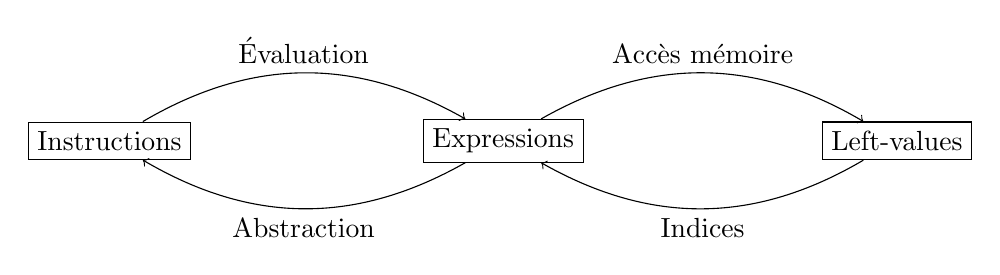
\begin{tikzpicture}
[node distance=5cm]

\node[draw] (I) {Instructions};

\node[draw, right of=I] (E) {Expressions};

\node[draw, right of=E] (L) {Left-values};

\draw[->] (I) edge[bend left] node[auto] {Évaluation} (E);
\draw[->] (E) edge[bend left] node[auto] {Abstraction} (I);
\draw[->] (E) edge[bend left] node[auto] {Accès mémoire} (L);
\draw[->] (L) edge[bend left] node[auto] {Indices} (E);

\end{tikzpicture}
\end{center}

\begin{theorem}[Progrès]
\label{thm:progres}

Supposons que $Γ ⊢ i$. Soit $m$ un état mémoire tel que $\mcomp{Γ}{m}$.

Alors l'un des cas suivants est vrai:
\begin{itemize}
\item $i = \iPass$
\item $∃v, i = \iReturn{v}$
\item $∃ (i', m'), \mm{m}{i}{m'}{i'}$
\item $∃ Ω ∈ \{\serr{div},\serr{array},\serr{ptr}\}, \msi{m}{i} → Ω$
\end{itemize}

\jolibreak

  Supposons que $Γ ⊢ e : t$. Soit $m$ un état mémoire tel que $\mcomp{Γ}{m}$.
  Alors l'un des cas suivant est vrai:

\begin{itemize}
  \item $∃ v ≠ Ω, e = v$
  \item $∃ (e', m'), \mm{m}{e}{m'}{e'}$
  \item $∃ Ω ∈ \{\serr{div},\serr{array},\serr{ptr}\}, \msi{m}{e} → Ω$
\end{itemize}

\jolibreak

Supposons que $Γ ⊢ lv : t$. Soit $m$ un état mémoire tel que $\mcomp{Γ}{m}$.

Alors l'un des cas suivants est vrai:
\begin{itemize}
\item $∃φ, lv = φ$
\item $∃ (lv', m'), \mm{m}{lv}{m'}{lv'}$
\item $∃ Ω ∈ \{\serr{div},\serr{array},\serr{ptr}\}, \msi{m}{lv} → Ω$
\end{itemize}

\end{theorem}

C'est-à-dire, soit:

\begin{itemize}
  \item l'entité (instruction, expression ou left-value) est complètement
évaluée.
  \item un pas d'évaluation est possible.
  \item une erreur de division, tableau ou pointeur se produit.
\end{itemize}

La preuve du théorème~\ref{thm:progres} se trouve en annexe~\ref{proof:progres}.

% TODO comm?
%\begin{lemma}[Permutation]
  %L'ordre dans lequel les variables apparaissent dans un environnement
  %n'influe pas sur la relation de typage.

  %Pour toute permutation $σ$ de $[1;n]$, on note $σ(x_1 : t_1, …, x_n : t_n) =
  %x_{σ(1)} : t_{σ(1)}, … x_{σ(n)} : t_{σ(n)}$.

  %Alors : si $Γ ⊢ e : t$ et $Γ' = σ(Γ)$, alors $Γ' ⊢ e : t$.
%\end{lemma}

%\begin{lemma}[Affaiblissement]
  %De même que l'ordre n'influe pas le typage, on peut aussi ajouter des
  %associations supplémentaires dans l'environnement sans modifier les typages
  %dans cet environnement.

  %Si $Γ ⊢ e : t$ et $x ∉ \cDom{Γ}$, alors $Γ, x : t' ⊢ e : t$.
%\end{lemma}

%\begin{lemma}[Substitution]
  %Si dans une expression $e$ il apparait une variable $x$ de type $t'$, le
  %typage est préservé lorsqu'on remplace ses occurrences par une expression $e'$
  %de même type.

  %Si $Γ, x : t' ⊢ e : t$ et $Γ ⊢ e' : t'$, alors $Γ ⊢ e [x/e'] : t$.
%\end{lemma}

%Ces lemmes permettent de prouver le théorème suivant :

\begin{theorem}[Préservation]
\label{thm:preservation}

Soient $Γ$ un environnement de typage, et $m$ un état mémoire tels que
$\mcomp{Γ}{m}$.

Alors:

\begin{itemize}
\item
    Si $Γ ⊢ e : t$ et $\mm{m}{e}{m'}{e'}$,
    alors $\mcomp{Γ}{m'}$ et $Γ ⊢ e' : t$.

\item
    Si $Γ ⊢ e : t$ et $\mm{m}{e}{m'}{v}$,
    alors $\mcomp{Γ}{m'}$ et $m ⊧ v : τ$ où $\tComp{τ}{t}$.
% TODO pê pas nécessaire d'avoir un m'

\item
    Si $Γ ⊢ i$ et $\mm{m}{i}{m'}{i'}$,
    alors $\mcomp{Γ}{m'}$ et $Γ ⊢ i'$.

\item
    Si $Γ ⊢ lv : t$ et $\mm{m}{lv}{m'}{lv'}$,
    alors $\mcomp{Γ}{m'}$ et $Γ ⊢ lv' : t$.

% TODO un cas avec les lv → φ?
\end{itemize}

  Autrement dit, si une construction est typable, alors un pas d'évaluation ne
  modifie pas son type et préserve le typage de la mémoire.

\end{theorem}

La preuve de ce théorème se trouve en annexe~\ref{proof:preservation}.

Cela prouve qu'aucun terme ne reste ``bloqué'' parce qu'aucune règle ne
s'applique, et que la sémantique respecte le typage. En quelque sorte, les types
sont un contrat entre les expressions et les fonctions: si leur évaluation
converge, alors une valeur du type inféré sera produite.

Enfin, on donne une version de ces propriétés pour les phrases de programme.

\begin{theorem}[Progrès pour les phrases]

Soient $Γ$ un environnement de typage, $m$ un état mémoire et $p$ une phrase de
programme. Supposons que $\typh{Γ}{p}{Γ'}$ et $\mcomp{Γ}{m}$.

On suppose en outre que l'évaluation de $p$ termine.

Alors $∃ m'. \ph{m}{p}{m'}$.

% TODO passer à un plus petit pas.

\end{theorem}

\begin{proof}

On distingue selon la dernière règle de typage appliquée dans la dérivation de
$\typh{Γ}{p}{Γ'}$.

\paragraph{\textsc{T-Exp}:} % {{{

On applique le théorème de progrès à $e$. Puisque l'évaluation termine, il
existe $v$ et $m'$ tels que $\mm{m}{e}{m'}{v}$. Alors on peut appliquer
\textsc{T-Exp}.

%}}}
\paragraph{\textsc{T-Var}:} % {{{
Idem avec \textsc{T-Var}.
%}}}

\end{proof}

\begin{theorem}[Préservation pour les phrases]

On suppose que les trois propriétés suivantes sont vérifiées:

\[
\begin{cases}
    \mcomp{Γ}{m} \\
    \typh{Γ}{p}{Γ'} \\
    \ph{m}{p}{m'}
\end{cases}
\]

Alors $\mcomp{Γ'}{m'}$.

\end{theorem}

\begin{proof}
% TODO
\end{proof}

% vim: spelllang=fr
